\documentclass[
	% -- opções da classe memoir --
	12pt,				% tamanho da fonte
	openright,			% capítulos começam em pág ímpar (insere página vazia caso preciso)
	oneside,			% para impressão em frente e verso. Oposto a oneside
	a4paper,			% tamanho do papel.
	% -- opções da classe abntex2 --
	chapter=TITLE,		% títulos de capítulos convertidos em letras maiúsculas
	section=TITLE,		% títulos de seções convertidos em letrashttps://www.overleaf.com/project/5e94d40a085e6600014b4986 maiúsculas
	subsection=TITLE,	% títulos de subseções convertidos em letras maiúsculas
	subsubsection=TITLE,% títulos de subsubseções convertidos em letras maiúsculas
	% -- opções do pacote babel --
	english,			% idioma adicional para hifenização
	brazil				% o último idioma é o principal do documento
	]{abntex2}


% ---
% Pacotes básicos 
% ---
%\usepackage{lmodern}			% Usa a fonte Latin Modern
\usepackage{mathptmx}			% Usa a fonte Times New Roman
%\usepackage{helvet}			% Fonte Parecida com Arial
\usepackage[T1]{fontenc}		% Selecao de codigos de fonte.
\usepackage[utf8]{inputenc}		% Codificacao do documento (conversão automática dos acentos)
\usepackage{lastpage}			% Usado pela Ficha catalográfica
\usepackage{indentfirst}			% Indenta o primeiro parágrafo de cada seção.
\usepackage{color}				% Controle das cores
\usepackage{graphicx}			% Inclusão de gráficos
\usepackage{subcaption}			% Inclusão de gráficos lado a lado
\usepackage{microtype} 			% para melhorias de justificação
\usepackage{tabularx,ragged2e}	% Para inserir tabelas
\usepackage{multirow}			% Para mesclar células
\usepackage[dvipsnames,table,xcdraw]{xcolor}		% Permite adicionar cores nas linhas de tabelas
\usepackage{fancyvrb}			% Permite adicionar arquivos de texto
\usepackage[portuguese, ruled, linesnumbered]{algorithm2e} % Uso de algoritmos
\usepackage{amsfonts}			% Permite usar notação de conjuntos
\usepackage{amsmath}			% Permite citar equações
\usepackage{amsthm}				% Permite criar teoremas e experimentos
\usepackage[font={bf, small}, labelsep=endash, labelfont=bf]{caption}	% Faz legenda de figuras ficarem em negrito
\usepackage{cancel}				% Permite fazer expressão tendendo a zero
\usepackage{epstopdf}			% Converte eps para pdf
\usepackage[final]{pdfpages}
\usepackage{hyphenat}
\usepackage{fancyhdr}
\usepackage{longtable}
\usepackage{graphicx}

\newcolumntype{L}{>{\RaggedRight\arraybackslash}X}
% ---
		
% ---
% Pacotes adicionais, usados apenas no âmbito do Modelo Canônico do abnteX2
% ---
\usepackage{lipsum}				% para geração de dummy text
% ---

% ---
% Pacotes de citações
% ---
%\usepackage[brazilian,hyperpageref]{backref}	 % Paginas com as citações na bibl
\usepackage[alf, abnt-emphasize=bf]{abntex2cite}	% Citações padrão ABNT

% ---
% Customizações para o layout da UFPA
% ---
\usepackage{modelo-ufpa/ufpa}

\tolerance=1
\emergencystretch=\maxdimen
\hyphenpenalty=10000
\hbadness=10000
\hyphenchar\font=-1
\sloppy
\renewcommand{\ABNTEXchapterfontsize}{\normalsize}
\renewcommand{\ABNTEXsectionfontsize}{\normalsize}
\renewcommand{\ABNTEXsubsectionfontsize}{\normalsize}
\renewcommand{\ABNTEXsectionfont}{}
\renewcommand{\ABNTEXsubsectionfont}{}

\renewcommand{\chaptername}{ }
%\renewcommand{\familydefault}{\sfdefault} % usar apenas se usar a fonte helvet

% Muda o título de lista de ilustrações para lista de figuras
\addto\captionsbrazil{%
  \renewcommand{\listfigurename}%
    {Lista de Ilustrações}%
	\renewcommand{\listtablename}%
    {Lista de Tabelas}%
}

\fancypagestyle{ultima}{
\fancyhead{}
\fancyfoot{}
\rhead{\thepage}
}

% Permite utilizar figuras sem precisar colocar o caminho absoluto
\graphicspath{{imagens/}}

% Define o ambiente de experimentos
\theoremstyle{definition}
\newtheorem{experimento}{Experimento}[section]
\newcommand{\experimentoautorefname}{Experimento}

% --- 
% CONFIGURAÇÕES DE PACOTES
% --- 

% ---
% Configurações do pacote backref
% Usado sem a opção hyperpageref de backref
%\renewcommand{\backrefpagesname}{Citado na(s) página(s):~}
% Texto padrão antes do número das páginas
%\renewcommand{\backref}{}
% Define os textos da citação
%\renewcommand*{\backrefalt}[4]{
%	\ifcase #1 %
%		Nenhuma citação no texto.%
%	\or
%		Citado na página #2.%
%	\else
%		Citado #1 vezes nas páginas #2.%
%	\fi}%
% ---

% ---
% Informações de dados para CAPA, FOLHA DE ROSTO e FICHA CATALOGRÁFICA
% ---
\universidade{CENTRO UNIVERSITÁRIO SERRA DOS ÓRGÃOS - UNIFESO}
\instituto{CENTRO DE CIÊNCIA E TECNOLOGIA - CCT}
\curso{CURSO DE BACHARELADO EM CIÊNCIA DA COMPUTAÇÃO}
% \titulo{TESTES AUTOMATIZADOS DE ACESSIBILIDADE NA WEB: UM ESTUDO DE CASO DO AMBIENTE VIRTUAL DE APRENDIZAGEM DO UNIFESO}
% opção 2 de título
% ---
\titulo{TESTES AUTOMATIZADOS DE ACESSIBILIDADE NA WEB: \\UM ESTUDO DE CASO DO AVA DO UNIFESO}
% ---
\autor{Lucas da Silva Cruz}
\local{TERESÓPOLIS}
\data{2021}
\orientador{Prof. Nelson Ned Nascimento Lacerda}
%\coorientador{Prof. NOME DO COORIENTADOR} %CASO HAJA UM
\tipotrabalho{Monografia}
\preambulo{Trabalho de Conclusão de Curso apresentado ao Centro Universitário Serra dos Órgãos como requisito obrigatório para obtenção do título de Bacharel em Ciência da Computação.}
\sobrenome{da Silva Cruz}
\nome{Lucas}% APENAS O PRIMEIRO NOME SEM SOBRENOME
\palavraschave{%
Acessibilidade,
\textit{e-Learning},
Testes automatizados,
WCAG,
AVA.
}

\datadadefesa{Data da Defesa: 28 de Novembro de 2020}% PREENCHER COM O DATA DA DEFESA}
%\conceito{Conceito: Excelente}
\faculdadedoorientador{FACULDADE DO ORIENTADOR} %
\titulacaodoorientador{DSc}%Coloque abreviado a titulação do seu Orientador
\primeiromembrodabanca{Prof. Rafael Monteiro}
\titulacaodoprimeiromembro{MSc}
\faculdadedoprimeiromembrodabanca{UNIFESO}
\segundomembrodabanca{Prof. Hermano Lustosa}
\titulacaodosegundomembro{DSc}
\faculdadedosegundomembrodabanca{UNIFESO}
% ---

% ---
% Configurações de aparência do PDF final

% alterando o aspecto da cor azul
\definecolor{blue}{RGB}{41,5,195}

% informações do PDF

\makeatletter
\hypersetup{
     	%pagebackref=true,
		pdftitle={\imprimirtitulo}, 
		pdfauthor={\imprimirautor},
    	pdfsubject={\imprimirpreambulo},
	    pdfcreator={LaTeX with abnTeX2},
		pdfkeywords={\imprimirpalavraschave}, 
		colorlinks=true,       		% false: boxed links; true: colored links
    	linkcolor=black,          	% color of internal links
    	citecolor=black,        		% color of links to bibliography
    	filecolor=magenta,      		% color of file links
		urlcolor=black,
		bookmarksdepth=4,
        breaklinks=true
}
\makeatother


% --- 

% --- 
% Espaçamentos entre linhas e parágrafos 
% --- 

% O tamanho do parágrafo é dado por:
\setlength{\parindent}{1.5cm}

% Controle do espaçamento entre um parágrafo e outro:
\setlength{\parskip}{0.2cm}  % tente também \onelineskip

% ---
% compila o indice
% ---
\makeindex
% ---

% ----
% Início do documento
% ----
\begin{document}

\nocite{Vrs:2018}
% Seleciona o idioma do documento (conforme pacotes do babel)
%\selectlanguage{english}
\selectlanguage{brazil}

% Retira espaço extra obsoleto entre as frases.
\frenchspacing 


% ----------------------------------------------------------
% ELEMENTOS PRÉ-TEXTUAIS
% ----------------------------------------------------------
% \pretextual

% ---
% Capa
% ---
\imprimircapa
% ---

% ---
% Folha de rosto
% ---
\imprimirfolhaderosto
% ---

% ---
% Inserir a ficha bibliografica
% ---
% A biblioteca da universidade lhe fornecerá um PDF
% com a ficha catalográfica definitiva após a defesa do trabalho. Quando estiver
% com o documento, salve-o como PDF no diretório do seu projeto e substitua todo
% o conteúdo de implementação deste arquivo pelo comando abaixo:

% \begin{fichacatalografica}
%     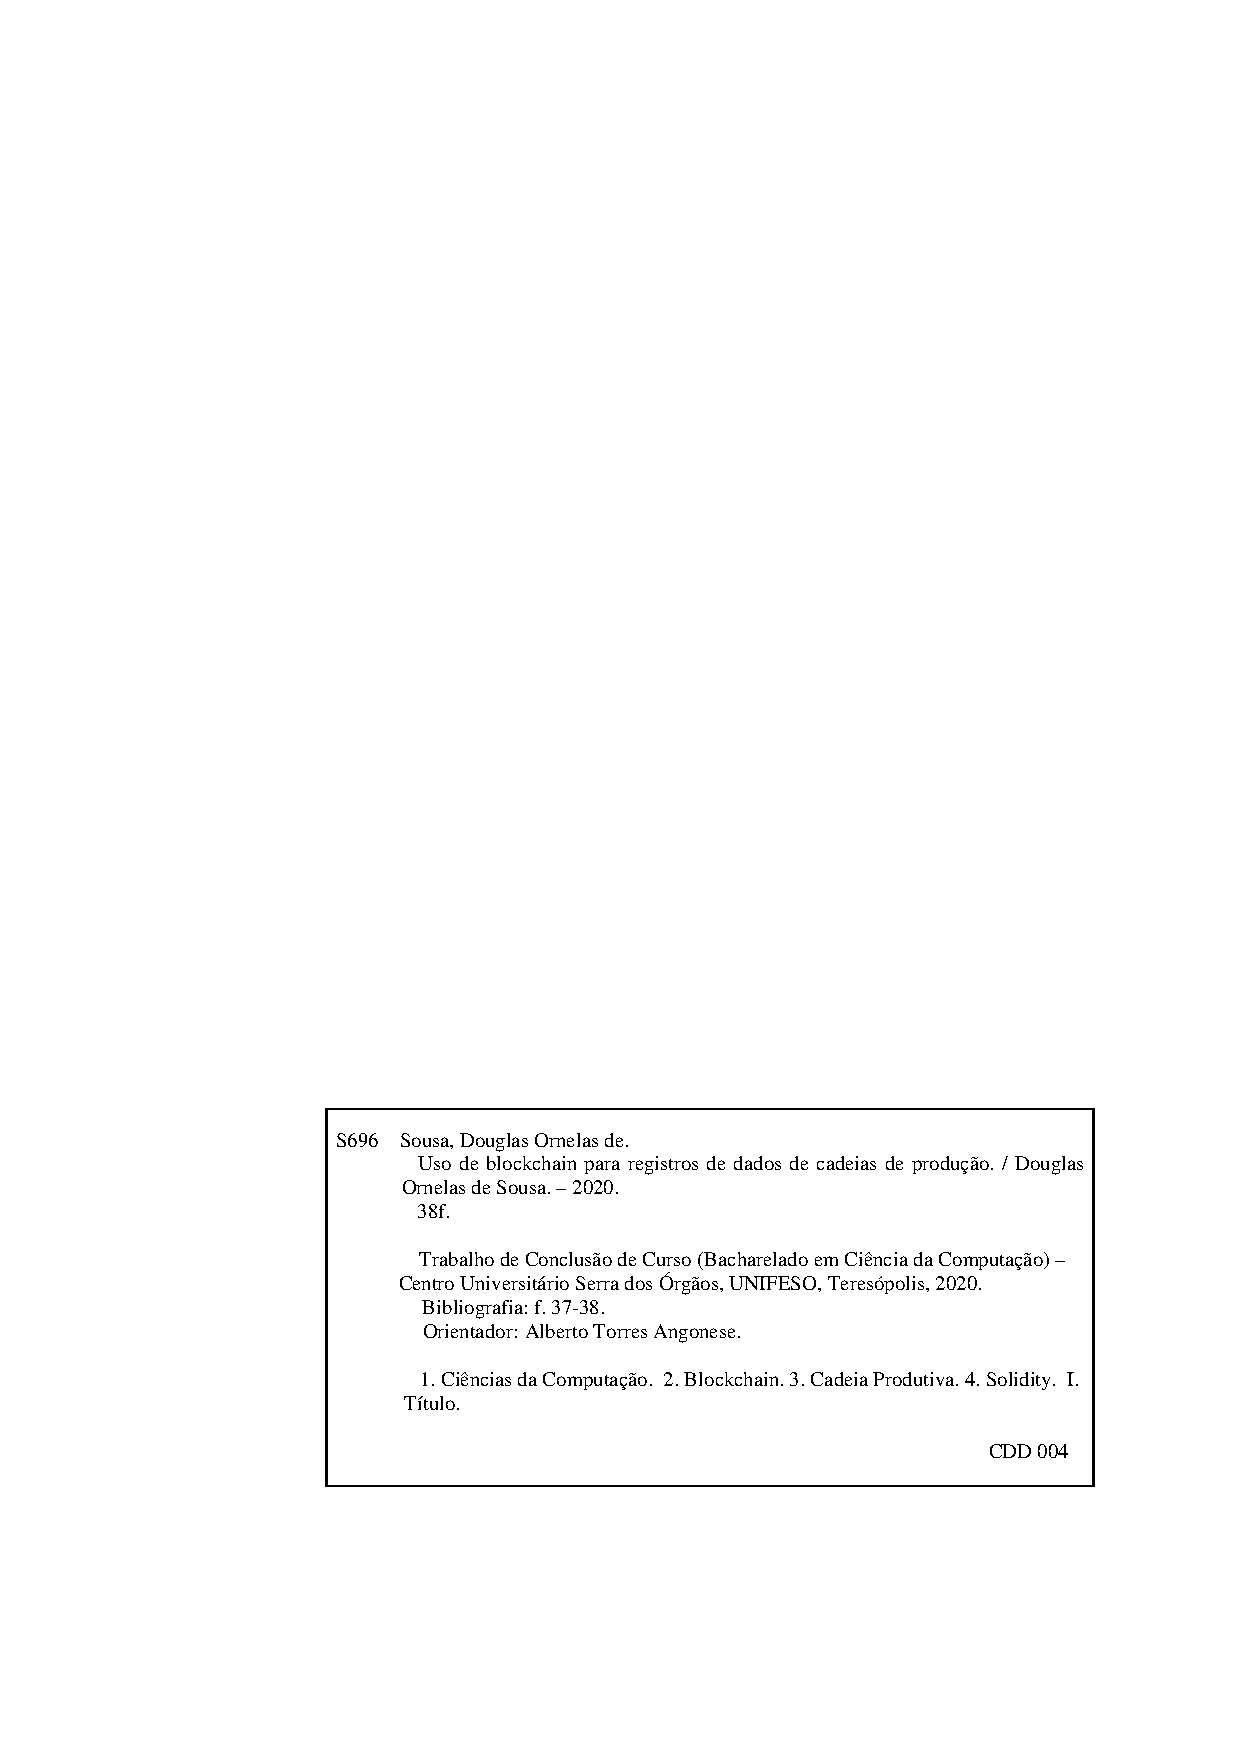
\includepdf{fichacatalografica.pdf}
% \end{fichacatalografica}


\newpage
% ---
% ---

% ---
% Inserir folha de aprovação
% ---
%
\begin{folhadeaprovacao}
\imprimirfolhadeaprovacao
\end{folhadeaprovacao}


% ---

% ---
% Dedicatória
% ---

% ESCREVA A SUA DEDICATORIA A DEDICATORIA QUE SE ENCONTRA NO ARQUIVO E APENAS UM EXEMPLO. ESCOLHA A DEDICATORIA QUE MAIS LHE AGRADAR. LEMBRE-SE DE UTILIZAR AS '\\' PARA PULAR LINHAS

\begin{dedicatoria}
   \vspace*{\fill}
   \flushright
   %\noindent
   \textit{Aos meus pais, que me deram todas as oportunidades \\e incentivos para estudar que eles mesmos não tiveram.}
\end{dedicatoria}
% ---

% ---
% Agradecimentos
% ---
\begin{agradecimentos}

Antes de mais nada quero agradecer principalmente a minha família por todo apoio, participação e incentivo durante todo meu processo de formação. À minha companheira de longo prazo, Sarah de Almeida Ferreira, por sempre me ajudar e socorrer nos momentos mais difíceis da minha vida. Agradeço a todos os meus professores e professoras desde a escola à graduação, ao Centro Universitário Serra dos Órgãos (Unifeso) por todas as oportunidades, experiências e pelo ambiente acolhedor que se tornou a minha segunda casa. Um agradecimento especial aos profs. Tiago Resende e Nelson Lacerda pela impecável disponibilidade e paciência na execução de todo este trabalho.

% A todos que, direta ou indiretamente, colaboraram para a realização desta monografia. 

\end{agradecimentos}
% ---

% ---
% Epígrafe
% ---

% ESCREVA A SUA EPÍGRAFE A MESMA QUE SE ENCONTRA NO ARQUIVO E APENAS UM EXEMPLO. ESCOLHA A EPÍGRAFE QUE MAIS LHE AGRADAR. LEMBRE-SE DE UTILIZAR AS '\\' PARA PULAR LINHAS

\begin{epigrafe}
    \vspace*{\fill}
	\begin{flushright}
		\textit{``A criatividade pode ser uma contribuição social, \\ mas apenas na medida em que a sociedade é livre para usar os resultados.''\\
		(Richard Stallman)}
	\end{flushright}
\end{epigrafe}
% ---

% ---
% RESUMOS
% ---

% resumo em português
\setlength{\absparsep}{18pt} % ajusta o espaçamento dos parágrafos do resumo
\begin{resumo}

As Tecnologias de Informação e Comunicação (TIC) são elementos fundamentais e determinantes para criação de práticas mais democráticas. No âmbito da educação, os Ambientes Virtuais de Aprendizagem (AVA) têm se mostrado um importante instrumento na propagação de conhecimento para aqueles que historicamente não teriam acesso ao ensino, como as pessoas portadoras de alguma deficiência. No entanto, quando o acesso a essas tecnologias não se dá de forma uniforme é criado um fenômeno de marginalização informacional. O presente trabalho discorre sobre a utilização de testes automatizados de acessibilidade como forma de validar requisitos fundamentais recomendados pelas Diretrizes de Acessibilidade para o Conteúdo da Web (WCAG), realizando um estudo de caso do AVA usado no Centro Universitário Serra dos Órgãos (Unifeso) e considerando que os métodos e resultados documentados nesta auditoria possam ser reutilizados em outros \textit{e-Learnings}, popularizarados devido à digitalização intensificada pelo confinamento – principal meio de controle do coronavírus.

 \textbf{Palavras-chave}: \imprimirpalavraschave
\end{resumo}

% resumo em inglês
\begin{resumo}[Abstract]
 \begin{otherlanguage*}{english}
  
Information and Communications Technology (ICT) are fundamental and determinant elements to build more democratic practices. In the field of education, Virtual Learning Environments (VLE) have proven to be an important tool in the dissemination of knowledge to those who historically would not have access to education, such as people with disabilities. However, when access to these technologies is not uniform, a phenomenon of informational marginalization is created. This undergraduate thesis discusses the use of automated accessibility tests as a way to validate fundamental requirements recommended by the Web Content Accessibility Guidelines (WCAG), performing a case study of the VLE used at the Serra dos Órgãos University Center (Unifeso) and considering that the methods and results documented in this audit can be reused in other e-Learnings, popularized due to digitization intensified by confinement – the main means of controlling coronavirus.

   \vspace{\onelineskip}
 
   \noindent 
   \textbf{Keywords}: Accessibility, e-Learning, Test automation, WCAG, AVA.
 \end{otherlanguage*}
\end{resumo}

% ---

% ---
% inserir lista de ilustrações
% ---
% UTILIZE CASO HAJA FIGURAS NA MONOGRAFIAS. EM QUASO DE AUSENCIA DE FIGURAS COMENTAR COM AS 3 LINHAS DE CODIGOS UTILIZANDO O '%'.
\pdfbookmark[0]{\listfigurename}{lof}
\listoffigures*
\cleardoublepage
% ---

% ---
% inserir lista de quadros
% ---
% UTILIZE CASO HAJA QUADROS NA MONOGRAFIAS. EM QUASO DE AUSENCIA DE QUADROS COMENTAR COM AS 3 LINHAS DE CODIGOS UTILIZANDO O '%'.

%\pdfbookmark[0]{\listofquadrosname}{loq}
%\listofquadros*
%\cleardoublepage
% ---

% ---
% inserir lista de tabelas
% ---

% UTILIZE QUASE HAJA TABELAS NA MONOGRAFIAS. EM QUASO DE AUSENCIA DE TABELAS COMENTAR COM AS 3 LINHAS DE CODIGOS UTILIZANDO O '%'.

%\pdfbookmark[0]{\listtablename}{lot}
%\listoftables*
%\cleardoublepage
% ---

% ---
% inserir lista de algoritmos
% ---

% UTILIZE CASO HAJA ALGORITMOS NA MONOGRAFIAS. EM QUASO DE AUSENCIA DE ALGORITMOS COMENTAR COM AS 3 LINHAS DE CODIGOS UTILIZANDO O '%'.

%\pdfbookmark[0]{\listalgorithmcfname}{loa}
%\imprimirlistadealgoritmos
%\cleardoublepage
% ---

% ---
% inserir lista de abreviaturas e siglas
% ---
% DEVE SER PREENCHIDA A MÃO LEMBRE-SE DE MANTER EM ORDEM ALFABETICA.
%\begin{siglas}
%  \item[ABNT] Associação Brasileira de Normas Técnicas
%\end{siglas}
% ---

% ---
% inserir lista de símbolos
% ---
% DEVE SER PREENCHIDA A MÃO LEMBRE-SE DE MANTER EM ORDEM ALFABETICA.
%\begin{simbolos}
%  \item[$ \theta $] Letra grega maiúscula theta
%\end{simbolos}
% ---



% ---
% inserir o sumario
% ---
\pdfbookmark[0]{\contentsname}{toc}
\tableofcontents*
\cleardoublepage
% ---



% ----------------------------------------------------------
% ELEMENTOS TEXTUAIS
% ----------------------------------------------------------
\textual
\pagestyle{simple}

% ----------------------------------------------------------
% Introdução
% ----------------------------------------------------------
\chapter{INTRODUÇÃO}

Vivemos em um tempo de explosão informacional onde as Tecnologias de Informação e Comunicação (TIC) se tornaram elementos fundamentais e determinantes para a criação de práticas mais democráticas. Nesse contexto contemporâneo, o direito à comunicação e à informação, bem como a democratização das TICs, são fundamentais \cite{morigireencantamento}.

Por outro lado, quando o acesso às tecnologias não se dá de forma uniforme é criado um fenômeno de "marginalização informacional", como afirmado em  \cite{matellart2002historia}. Em \cite{esteves2010novos}, essa exclusão social compreende uma nova versão do “digital divide”, que evidencia como as diferenças de acesso refletem as reais desigualdades sociais, políticas e econômicas entre a população incluída e excluída digitalmente.

Apesar do tema Inclusão Social e Digital vir sendo objeto de debates no meio acadêmico, governamental e empresarial, a questão da inclusão de pessoas portadoras de necessidades especiais, em todos os recursos da sociedade, ainda é muito incipiente no Brasil \cite{maciel2000portadores}. Uma das formas de exclusão digital está associada justamente à falta de acessibilidade nos serviços e informações da Web, embora ela tenha sido projetada para ser utilizada por qualquer pessoa. As Diretrizes de Acessibilidade para Conteúdo Web (WCAG) visam fornecer recomendações que tornem o conteúdo acessível a um maior número de pessoas com deficiência, que incluem:

\begin{citacao}
“acomodações para cegueira e baixa visão, surdez e baixa audição, limitações de movimentos, incapacidade de fala, fotossensibilidade e combinações destas características, e alguma acomodação para dificuldades de aprendizagem e limitações cognitivas; mas não abordará todas as necessidades de usuários com essas deficiências. Seu conteúdo da Web também ficará mais acessível aos usuários em geral ao seguir estas diretrizes.” \cite{caldwell2008web}
\end{citacao}

Nos dias atuais, é uma prática intrínseca ao desenvolvimento de um Sistema Web garantir a sua usabilidade, que pode ser definida como o fator que assegura que um produto ou serviço seja fácil de usar, eficiente e agradável a partir do ponto de vista do usuário \cite{sharp2005design}. Porém, em relação a acessibilidade, que considera a diversidade de seus possíveis usuários e as peculiaridades da interação dessas pessoas com o produto \cite{torres2004conteudos}, muitas das vezes os desenvolvedores e especialistas em Garantia de Qualidade (QA) não consideram as diretrizes e padrões da WCAG no design e na \textit{test suite} (conjunto de casos de teste) das aplicações, gerando uma série de problemas para o usuário com alguma deficiência.

Por causa disso surgiram as \textit{engines} como Axe e Pa11y, que implementam as regras da WCAG e rodam testes automatizados de acessibilidade nas páginas de uma aplicação da web. Elas foram arquitetadas e desenvolvidas para integrar com qualquer ambiente de teste já existente em um projeto, de forma que as organizações possam automatizar os testes de acessibilidade junto dos seus testes regulares.

Essas ferramentas foram utilizadas neste trabalho para realizar um estudo de caso no Ambiente Virtual de Aprendizagem (AVA) do Centro Universitário Serra dos Órgãos (Unifeso), com o intuito de explicitar as formas mais modernas de se realizar testes automatizados de acessibilidade em e-Learnings e, com isso, alcançar práticas mais democráticas no acesso ao ensino e às tecnologias por pessoas portadoras de alguma deficiência.


\section{Justificativa}

A adoção de medidas de confinamento para diminuir a velocidade de propagação do coronavírus fez com que muitas instituições enfrentassem uma digitalização forçada. Com o aumento na utilização das TIC também foi evidenciado a falta de acessibilidade nos serviços e informações da Web, embora ela tenha sido projetada para ser utilizada por qualquer pessoa. No âmbito educacional, os AVAs foram muito utilizados para dar continuidade às atividades escolares e acadêmicas. Eles têm se mostrado um importante instrumento na propagação de conhecimento para aqueles que historicamente não teriam acesso a educação seja por questões financeiras, físicas ou de tempo \cite{sharma2014quantitative}. Assim, a validação da acessibilidade nas aplicações da web se mostra um desafio extremamente importante para criação de práticas mais democráticas. Além disso, seguir as WCAG deixa os sistemas não apenas mais usáveis para pessoas com alguma deficiência como também para usuários no geral. Hoje, com as modernas ferramentas de avaliação automática pode-se testar e garantir um bom nível de acessibilidade nos ambientes virtuais, aumentando também a qualidade dos sistemas para todos os usuários.
    
\section{Motivação}

Desenvolver softwares de valor e com qualidade para os usuários tem sido um desafio constante em tempos de agilidade. As organizações e pesquisadores tendem a associar as metodologias ágeis com a usabilidade e a Experiência do Usuário (UX), a fim de criar um modelo que promova este tipo de entrega. A acessibilidade também é um tópico crucial para todos os envolvidos no processo de desenvolvimento de uma aplicação na medida em que alguns usuários são completamente excluídos da experiência sem ela. O relatório sobre deficiência da Organização Mundial da Saúde (OMS) mostrou que mais de 1 bilhão da população mundial (15\%) vive com alguma forma de deficiência \cite{schiariti2020human}. Além da grande parcela que pode estar perdendo os aplicativos, geralmente encontrar e resolver problemas de acessibilidade beneficiam todos os usuários. Hoje, com a Computação em Nuvem, surge também um crescente interesse em projetos que visam abranger todos os aspectos da qualidade de um app da Web. Com essas ferramentas, testar e garantir um bom nível de acessibilidade não é uma tarefa complexa mas com certeza é um fator crucial e determinante
para criação de práticas mais democráticas.
    
\section{Objetivo}
 
Nesta seção serão apresentados os objetivos gerais e específicos do trabalho

\subsection{Objetivos Gerais}

Utilizar ferramentas de avaliação automática para identificar e resolver problemas de acessibilidade no Ambiente Virtual de Aprendizagem (AVA) do Centro Universitário Serra dos Órgãos (Unifeso).

\subsection{Objetivos Específicos}

Apresentar as principais ferramentas de avaliação automática de acessibilidade para aplicações da web;
    
Verificar a pontuação do AVA da Unifeso em termos de experiência do usuário (UX) e acessibilidade através do Google Lighthouse;

Executar testes automatizados para identificar os problemas chaves de acessibilidade, mais frequentes e como estão distribuídos;

Levantar soluções para resolver as falhas de acessibilidade identificadas de modo a melhorar consideravelmente a pontuação de UX e acessibilidade do AVA.
    
%\section{Organização da monografia}


\chapter{TRABALHOS RELACIONADOS}

Neste capítulo será apresentada trabalhos relacionados encontrados durante o desenvolvimento deste trabalho.

% \section{\textit{An Agri-food Supply Chain Traceability System for
% China Based on RFID & Blockchain Technology}} 

% Criado para ajudar com o controle de cadeia de produção de produtos agrícolas na China, a proposta tem como objetivo o uso de sensores e tecnologia \textit{blockchain} para garantir a segurança de consumo desses alimentos. O trabalho propõe principalmente o uso de sensores RFID (Identificação por Radiofrequência), que são sensores conforme a Figura \ref{Sensor RFID} que capturam dados a partir de etiquetas eletrônicas ou RF tags e permitem o controle e visualização dos mesmos. A partir destes sensores seria feita a confirmação dos dados e os mesmos passariam a ser registrados em uma rede \textit{blockchain} \cite{tian2016agri}.

% Assim como neste trabalho, o trabalho relacionado consiste em um registro de dados em cadeias de uma rede \textit{blockchain} para com isso ter sua rastreabilidade, usando até mesmo de dados registrados por sensores, porém o mesmo foi desenvolvido para o uso do controle de uma produção agrícola somente.

% \begin{figure}[!h]
% \centering
% \caption{Exemplo de sensor e RF tag, usados em um microcontrolador Arduino}
% \fbox{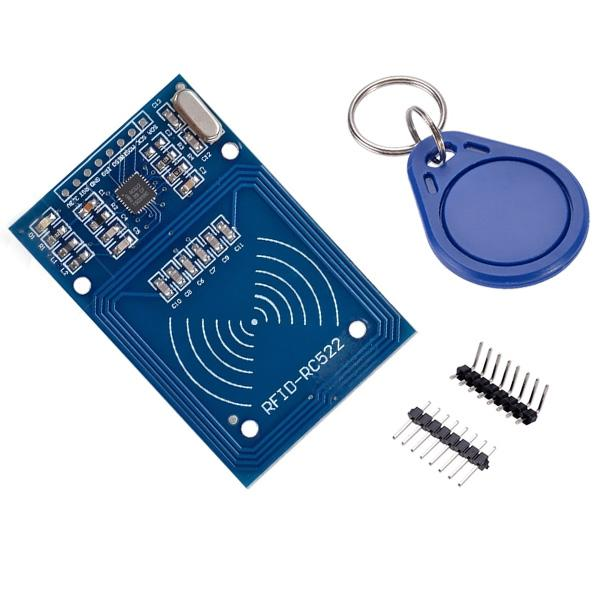
\includegraphics [scale=0.5]{trabalho_relacionado_1.jpg}}
% \legend{Fonte: \cite{MicroControlandos}}
% \label{Sensor RFID}
% \end{figure}

% \section{\textit{How blockchain improves the supply chain: case study alimentary supply chain}} 

% Proposta de modelo de cadeias de produção via \textit{blockchain}, com isso habilitando um economia circular e eliminando alguns problemas encontrados em cadeias de produção. Sua arquitetura pode ser vista na Figura \ref{Arquitetura Proposta pelo trabalho relacionado}, que mostra que cada uma de suas camadas se comunica a partir dos contratos inteligentes \cite{casado2018blockchain}.

% Embora a proposta seja semelhante à proposta levantada neste trabalho, a mesma não mostrava uma implementação de como seria feita, e sua estrutura de dados é baseada em um modelo circular para melhoria de registro de dados em qualquer cadeia de produção. 

% \begin{figure}[!h]
% \centering
% \caption{Arquitetura Proposta pelo trabalho relacionado}
% \fbox{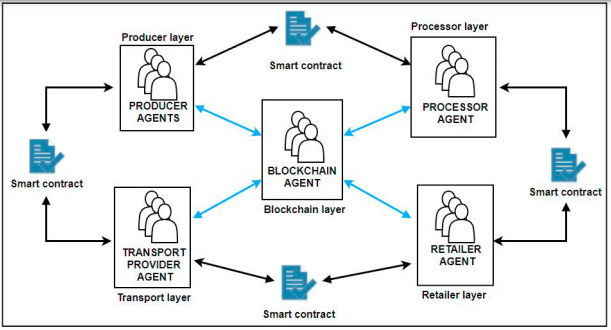
\includegraphics [scale=0.7]{trabalho_relacionado_2.png}}
% \legend{Fonte: \cite{casado2018blockchain}}
% \label{Arquitetura Proposta pelo trabalho relacionado}
% \end{figure}

% \section{QuipoAgro} 

% Produto criado para rastreabilidade de cadeias de produção de café, o mesmo possui o armazenamento de dados de etapas de produção de café e faz o registro das mesmas em rede \textit{blockchain}, conforme a Figura \ref{Interface QuipoAgro} \cite{QuipoAgro}.

% \begin{figure}[!h]
% \centering
% \caption{Interface QuipoAgro}
% \fbox{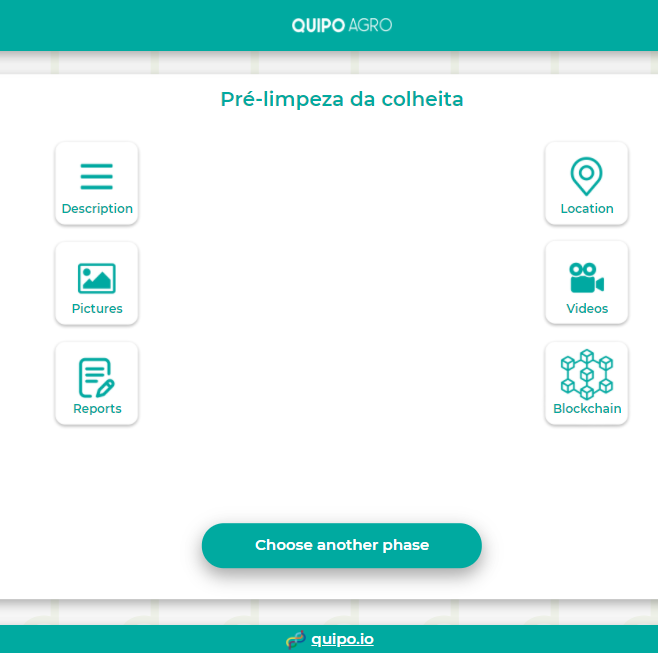
\includegraphics [scale=0.8]{Interface_QuipoAgro.PNG}}
% \legend{Fonte: agro.quipo.io/bt/1}
% \label{Interface QuipoAgro}
% \end{figure}

% O produto apresenta um funcionamento que se assemelha a forma que é desejada para o protótipo desenvolvido durante este trabalho, porém com a principal diferença sendo a permissão do envio de arquivos somente em um formato específico, enquanto o protótipo desenvolvido durante neste trabalho visa a permissão de dados para cadeias generalizadas.

% \begin{figure}[!h]
% \centering
% \caption{Comparação entre trabalhos relacionados}
% \fbox{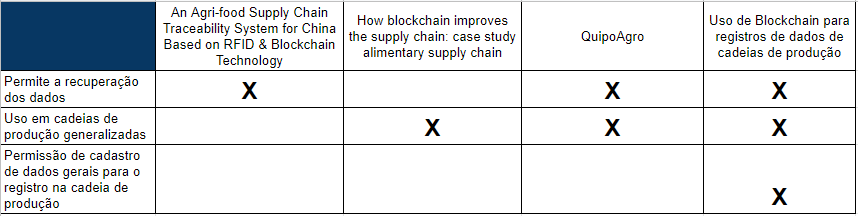
\includegraphics [scale=0.7]{Comparacao_trabalhos_relacionados.PNG}}
% \legend{Fonte: Autoria Própria}
% \label{Comparação entre trabalhos relacionados}
% \end{figure}


\chapter{FUNDAMENTAÇÃO TEÓRICA}

Em 2019 a Educação a Distância (EaD) tinha mais de 3,5 milhões de pessoas matriculadas em cursos superiores, segundo o relatório do Censo Nacional da Educação Superior publicado em 2020 \cite{da2019notas}. Para oferta dos cursos a distância ou até mesmo como forma de apoiar o ensino presencial as universidades têm adotado o modelo de e-Learning, comumente denominado de Ambiente Virtual de Aprendizagem (AVA). Com isso, os AVAs têm se mostrado um importante instrumento na propagação de conhecimento para aqueles que historicamente não teriam acesso a educação seja por questões financeiras, físicas ou de tempo \cite{sharma2014quantitative}.

Apesar disso, embora a EaD seja uma proposta de democratização do ensino, e as pessoas com deficiência estejam amparadas pelas leis para acesso à educação, no Brasil, a prática da acessibilidade ainda é reduzida \cite{dos2021acessibilidade}.

% [incluir considerações dos impactos do covid-2019 e digitalização forçada das universidades, ead temporário e tudo mais que fez usarmos mais AVAs e evidenciar o problema com deficientes em AVAs não muito acessíveis]

Para fornecer recomendações que tornem o conteúdo nos serviços e informações da Web mais acessível a um maior número de pessoas com deficiência foram criadas as Diretrizes de Acessibilidade para Conteúdo Web (WCAG). Assim, podemos testar se os AVAs foram desenvolvidos de forma a incluir os mais diversos tipos de usuário, seja com deficiência visual, auditiva, física, de fala, intelectual, de linguagem, de aprendizagem e neurológica \cite{caldwell2008web}.

\section{WCAG}
 
As Diretrizes de Acessibilidade para Conteúdo Web (WCAG) são um conjunto de recomendações para deixar a Web mais acessível. Seguir as diretrizes deixa não apenas mais usável para pessoas com alguma deficiência como também para usuários no geral. No documento é descrito vários critérios de sucesso sob a forma de declarações testáveis, especificados de forma que não dependem de nenhuma tecnologia específica e com informações de implementação e interpretação de cada critério de sucesso em documentos separados.

Para satisfazer as necessidades de diferentes grupos e situações foram definidos os chamados três níveis de conformidade: A, AA e AAA. O nível A atinge um nível mínimo de acessibilidade. Para atingir esse nível todos os critérios de sucesso do Nível A devem ser cumpridos e assim por diante nos outros níveis de conformidade. O nível AAA é o nível mais elevado e, em relação ao nível AA, esse é o nível considerado ideal, no qual o sistema atinge um nível fundamental de acessibilidade de modo que se torna acessível para a maioria das pessoas e na maior parte das situações, usando a maioria das tecnologias.

\pagebreak
 
\section{Testes Automatizados na Web}

Testar um software consiste em executá-lo de acordo como foi especificado, para determinar se ele irá comportar como esperado no ambiente para o qual ele foi projetado \cite{izabel2014testes}. Como a execução de todos os testes de forma manual é dispendiosa e requer muito tempo, é normal adotar abordagens automatizadas para isso.

Testes automáticos são executados por intermédio de um programa informático ou script, que é responsável pela comparação entre os resultados atuais e os esperados \cite{sharma2014quantitative}. Essa comparação é conhecida como assert: quando o resultado é diferente do esperado, o assert falha e seu valor é definido como falso; quando é igual, o teste passa e consideramos que a validação foi verdadeira.

No entanto, os testes automatizados para os AVAs requerem técnicas diferentes das aplicações tradicionais. Isto porque as técnicas tradicionais foram construídas pensando nas aplicações para desktop, uma vez que a Web foi inicialmente concebida como forma de publicação de hipertextos estáticos. Assim, as técnicas tradicionais não consideram características das aplicações web tais como a sua natureza multi-camada, estrutura baseada em hiperlink e dirigida a evento \cite{santa2011seleccao}.

Além disso, ao longo dos anos a própria Web sofreu sucessivas evoluções e modificações, apoiando aplicações de pequena e larga escala, desenvolvidas por equipes multidisciplinares com habilidades diversas e com emprego de novas e variadas tecnologias \cite{mendes2006need}, que aliadas à rápida evolução tecnológica proporciona novos desafios para as técnicas utilizadas no desenvolvimento de software \cite{santa2011seleccao}.

Em \cite{kappel2004web} foram representadas essas modificações categorizando as aplicações da web de forma a compreender melhor suas características e particularidades, a partir de um referencial histórico e por níveis de complexidade, onde as categorias mais novas são consideradas mais  complexas.

Na Figura \ref{Categorias de Aplicações Web} podemos observar as categorias de aplicações Web, com adaptação de ISABEL, que observa que as categorias mais recentes e consequentemente consideradas mais complexas são as aplicações ubíquas e as aplicações baseadas no conhecimento \cite{santa2011seleccao}.

\begin{figure}[!h]
\centering
\caption{Categorias de Aplicações Web}
\fbox{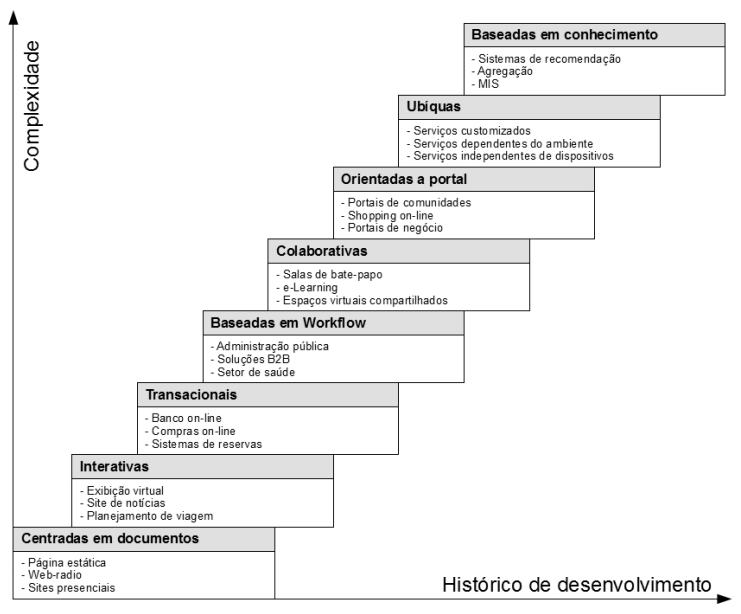
\includegraphics [scale=0.6]{Figura1.png}}
\legend{Fonte: \cite{santa2011seleccao}. Adaptado de \cite{kappel2004web}}
\label{Categorias de Aplicações Web}
\end{figure}

\pagebreak

\section{WebDriver e Selenium}

Pensando nessas características, com o intuito de evitar erros comuns nos sistemas da web, foram criados frameworks como o Selenium.

WebDriver é uma API e protocolo que define uma interface de linguagem neutra para manipular o comportamento dos navegadores. Cada implementação WebDriver específica de um navegador é chamada de driver – componente responsável por delegar ao navegador e pela comunicação do próprio navegador com o Selenium. Já o Selenium pode ser definido como um conjunto de diferentes ferramentas de software, onde cada uma possui um propósito específico para auxiliar no processo de automação de testes \cite{seleniumdoc}.

Na configuração do Selenium é definida e instalada as bibliotecas de linguagem – para linguagem escolhida do projeto de automação – e os binários dos drivers que executarão os testes no navegador. Graças a isso, além da possibilidade de ser controlado por diferentes linguagens de programação e frameworks de testes, o Selenium suporta a automação de praticamente todos os principais navegadores do mercado (Firefox, Google Chrome, Edge, Opera, Safari).

\section{Testes Automatizados de Acessibilidade}

Além dos frameworks voltados para testes automatizados na Web  também foram criados métodos para garantir uma melhor experiência do usuário nessas aplicações. Por exemplo, levando em consideração a usabilidade, que pode ser definida como o fator que assegura que um produto ou serviço seja fácil de usar, eficiente e agradável a partir do ponto de vista do usuário \cite{sharp2005design} temos as heurísticas de Nielsen, baseada em 294 tipos de erro de usabilidade que Jakob Nielsen, Ph.D., diretor da Nielsen Norman Group, encontrava em suas análises.

Mas em relação a acessibilidade, que considera a diversidade de seus possíveis usuários e as peculiaridades da interação dessas pessoas com o produto \cite{torres2004conteudos}, muitas das vezes os desenvolvedores e especialistas em Garantia de Qualidade (QA) não consideram as diretrizes e padrões da WCAG no design e na \textit{test suite} (conjunto de casos de teste) das aplicações, gerando uma série de problemas para o usuário com alguma deficiência.

Nesse contexto que surgiram as engines como Axe e Pa11y, que verificam se as regras da WCAG foram devidamente implementadas e executam testes automatizados de acessibilidade nas páginas de uma aplicação da web. Elas foram arquitetadas e desenvolvidas para integrar com qualquer ambiente de teste já existente em um projeto, de forma que as organizações possam automatizar os testes de acessibilidade junto dos seus testes regulares.

\section{Principais ferramentas automatizadas para testes de acessibilidade}

% [Caso seja melhor citar a page desatualizada do wcag das principais ferramentas para se automatizar e que essas, consideradas as melhores, foram retiradas de lá]:

\begin{itemize}

    \item aXe
    
O aXe é uma engine de testes de acessibilidade open-source para validação das recomendações sugeridas pela WCAG. Foi projetada para integrar com qualquer ambiente de teste existente, possibilitando a automatização dos testes de acessibilidade em conjunto com os testes funcionais regulares no processo de desenvolvimento de um sistema web. O aXe oferece uma série de ferramentas além da API (axe-core), como utilitários de CLIs (Interfaces de linha de comando) e a sua extensão para o Google Chrome.

A axe-core integra-se com o Selenium e funciona basicamente como uma ferramenta que definirá como automatizar os testes da página seguindo regras para o WCAG 2.0 e 2.1 nos níveis A e AAA. Com ela, é possível encontrar automaticamente em média 57\% dos problemas previstos no WCAG.
    
    \pagebreak
    
    \item Pa11y
    
O Pa11y também possui uma ferramenta CLI de teste de acessibilidade automatizado, que carrega páginas da web e destaca todos os problemas de acessibilidade encontrados. Além disso, também disponibiliza um serviço de Dashboard que faz os testes diariamente e ilustra melhor seus resultados para não-desenvolvedores, com gráficos que rastreiam melhorias e regressões ao longo do tempo. Esse painel também conta com um Webservice (Pa11y Webservice) baseado em JSON que dá suporte à criação de front-ends com o dashboard personalizado ou com redirecionamento dos dados.

    \item Google Lighthouse
    
O Google Lighthouse é uma ferramenta automatizada de código aberto que utiliza a biblioteca do aXe (axe-core) para fornecer um conjunto de testes de acessibilidade. Ela roda todas as regras marcadas com os tipos wcag2a e wcag2aa, apesar de desabilitar alguns itens específicos. O Lighthouse foi adicionada ao Chrome DevTools a partir da versão 60 do Google Chrome e também pode ser usado como uma ferramenta de linha de comando. Ele foi criada para oferecer uma auditoria abrangente de todos os aspectos de Qualidade de um app da Web.

\begin{figure}[!h]
\centering
\caption{Regras WCAG definidas no Lighthouse}
\fbox{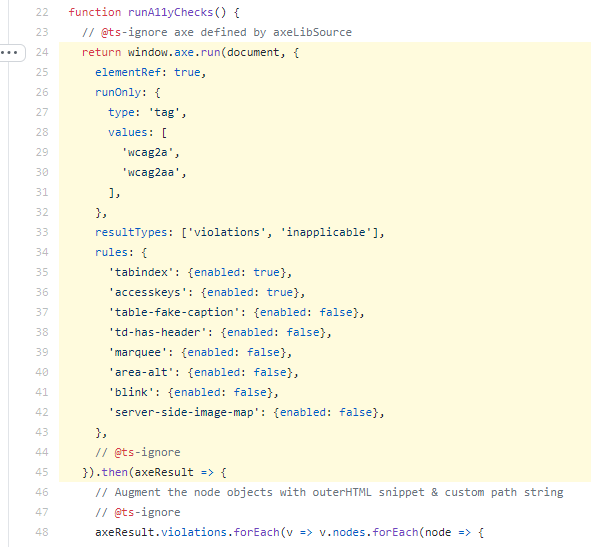
\includegraphics [scale=0.8]{Figura2.png}}
\legend{Fonte: Código retirado do \href{https://github.com/GoogleChrome/lighthouse/blob/b548452d8b0c3903d30c0effee0e10649ac8f5e6/lighthouse-core/gather/gatherers/accessibility.js}{repositório do Lighthouse} no Github. 2021.}
\label{Regras WCAG definidas no Lighthouse}
\end{figure}

\pagebreak

Atualmente, o Lighthouse cobre, além dos testes de acessibilidade, testes de desempenho, progressividade, boas práticas e SEO. A ferramenta também pode fazer testes para desktop ou mobile, no último caso usando emuladores de celular durante a auditoria.
    
\end{itemize}

\chapter{METODOLOGIA E DESENVOLVIMENTO}

Foi realizada uma pesquisa exploratória com o intuito de levantar procedimentos a serem adotados para se testar a acessibilidade de sistemas da Web. Com isso, o estudo foi realizado através das principais diretrizes e organizações de padronização que desenvolvem os pilares de tecnologias para se testar acessibilidade, de modo que antes de apurar as possíveis soluções sejam identificadas da melhor maneira possível as falhas de acessibilidade.

\section{Escopo e páginas da auditoria}

Foram analisadas 89 páginas do AVA a partir de um login com perfil de estudante. 178 testes automatizados foram executados – 1 por página – e encontradas, em um primeiro momento, um total de 600 falhas de acessibilidade. Ainda é preciso analisar as páginas com privilégio administrativo, disponíveis apenas no login de professores.

Em segunda instância, verificou-se que algumas páginas estavam sendo afetadas pelos mesmos componentes, o que causou duplicidades na análise ainda que os impactos na acessibilidade da plataforma afetem individualmente e repetitivamente a experiência do usuário com alguma deficiência. A pesquisa seguiu identificando em cada resultado por página, manualmente, os problemas de acessibilidade que já haviam sido acusados pelos testes em páginas anteriores. Foram consideradas duplicatas as análises sobre os mesmos componentes em duas páginas diferentes, que acusavam as mesmas vulnerabilidades. O mesmo tipo de falha de acessibilidade, encontrado em elementos distintos, também foi analisado separadamente considerando que apesar de ter a mesma solução ela deve ser aplicada em contextos diferentes, dependendo do elemento. Nessa fase, o total de falhas de acessibilidade passou a ser de 148 vulnerabilidades.

Durante a análise de duplicidade, os resultados também mostraram que a estrutura das páginas e seções é que continham os problemas de acessibilidade e não os dados ou valores taggeados. Com isso, foi revelado também que o mesmo tipo de página ou seção apresentavam os mesmos problemas de falha de acessibilidade ainda que fizesse parte de uma disciplina diferente. Por exemplo, a disciplina “2021/1 – DESENVOLVIMENTO DE APLICAÇÕES MÓVEIS” possuía as mesmas falhas de acessibilidade na seção Conteúdo das Aulas que a disciplina “2021/1 – COMPUTAÇÃO GRÁFICA E PROCESSAMENTO DE IMAGENS” na mesma seção. Ou seja, apesar dos testes automatizados terem sido executados em cima das disciplinas ofertadas para o 6º/7º período flex. das turmas semestrais de Ciência da Computação em 2021, os resultados cobrem todas as disciplinas do curso que apresentam as mesmas seções.


\section{Ferramentas utilizadas na avaliação}

\begin{itemize}

    \item Google Lighthouse
    
[escreva aqui]
    
    \item Chrome DevTools’ Color Picker
    
A ferramenta Chrome DevTools’ Color Picker possui uma integração com o Google Chrome, fazendo um link entre as análises automatizadas na guia do Lighthouse e facilitando a identificação e apuração do elemento com falha na acessibilidade na guia de elementos. Ela pode ser habilitada nas configurações do DevTools, na seção Experiments, como ilustrado mais abaixo na figura \ref{Habilitação da Chrome DevTools’ Color Picker no DevTools}.

\begin{figure}[!h]
\centering
\caption{Habilitação da Chrome DevTools’ Color Picker no DevTools}
\fbox{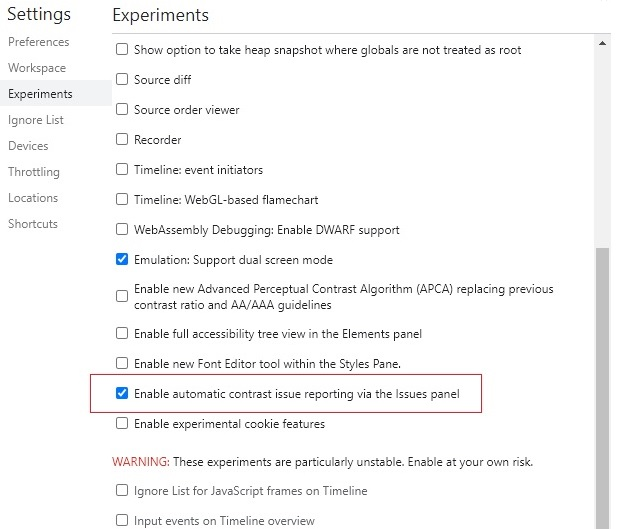
\includegraphics [scale=1.0]{Figura3.jpg}}
\legend{Fonte: Próprio autor}
\label{Habilitação da Chrome DevTools’ Color Picker no DevTools}
\end{figure}

Para utilização da ferramenta, depois de habilitada, basta inspecionar o elemento que terá a taxa de contraste apurada, identificar o valor de sua cor na guia Styles do DevTools e clicar na thumbnail à esquerda do valor. À direita do agrupamento Contrast ratio, poderá ser visualizada a taxa de contraste do elemento. Adiante na figura \ref{Apuração da taxa de contraste com o Chrome DevTools’ Color Picker } podemos visualizar como a ferramenta verifica o contraste sugerido pela WCAG no nível AA e no nível AAA, respectivamente.

\begin{figure}[!h]
\centering
\caption{Apuração da taxa de contraste com o Chrome DevTools’ Color Picker }
\fbox{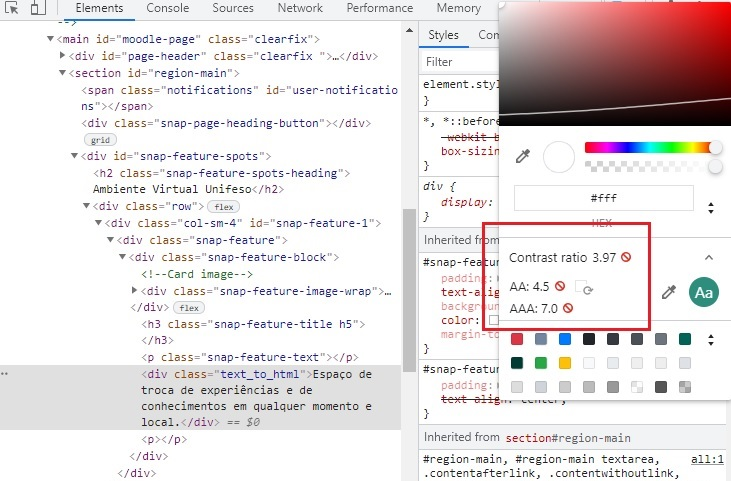
\includegraphics [scale=0.8]{Figura4.jpg}}
\legend{Fonte: Próprio autor}
\label{Apuração da taxa de contraste com o Chrome DevTools’ Color Picker }
\end{figure}

    \item Extensão Web Developer
    
[escreva aqui]
    
\end{itemize}

\chapter{RESULTADOS E DISCUSSÕES}

A avaliação identificou os problemas chaves de acessibilidade, mais frequentes e como estão distribuídos, que se relacionam com os fatores de pontuação e classificação de acessibilidade providos pelo próprio Google Lighthouse. No total, 12 asserts falharam.

\section{Sugestões de melhoria}

A partir desta apuração, foram levantadas para cada falha de acessibilidade uma proposta de solução que deve ser aplicada contextualmente a cada elemento acusado pelo Lighthouse com a mesma falha. As soluções, quando implementadas, impactariam consideravelmente a pontuação de acessibilidade do AVA, sendo esperada uma mudança na sua classificação de laranja para verde – considerada ideal pela ferramenta do Google.


\begin{itemize}

    \item ARIA input fields do not have accessible names
    
Esta falha de acessibilidade diz respeito aos elementos que não têm um valor de ARIA role apropriado e por isso não podem ser anunciados adequadamente aos usuários que utilizam leitores de tela. O Lighthouse tem algumas auditorias que cobrem um conjunto diferente de funções ARIA, dentre elas o conjunto conhecido como aria-input-field-name que cuida das roles combobox, listbox, searchbox, slider, spinbutton e textbox. Essa auditoria que, por exemplo, faz com que a div abaixo falhe no teste de acessibilidade.

\begin{center}
\begin{minipage}{10cm}
\begin{verbatim}
<div class="carousel-inner" role="listbox">
\end{verbatim}
\end{minipage}
\end{center}

O problema pode ser resolvido, conforme listado na seção 2.1, subtópico listbox \cite{world2014accessible}, adicionando o atributo aria-label ao elemento, que permite os leitores de tela e outras tecnologias assistivas anunciar seu valor para o usuário. Dessa forma, o problema acima poderia ser resolvido refatorando o exemplo da seguinte maneira:

\begin{center}
\begin{minipage}{10cm}
\begin{verbatim}
<div class="carousel-inner" role="listbox"
aria-label="Texto descritivo aqui">
\end{verbatim}
\end{minipage}
\end{center}
    
\pagebreak
    
    \item Elements with an ARIA [role] that require children to contain a specific [role] are missing some or all of those required children
    
Esta falha de acessibilidade acontece quando uma ARIA role é atribuída a um elemento com propósito de dizer aos leitores de tela e outras tecnologias assistivas qual o comportamento e os controles customizados que um componente da aplicação tem. Algumas dessas roles exigem que os filhos do elemento também tenham roles específicas que trabalham em conjunto com a do pai. Por exemplo, a role tablist exige que os filhos tenham a role tab.

Na figura \ref{Bloco de código pertencente à página inicial do AVA, mostrando a associação das roles listbox e options} podemos ver que a div acusada com falha de acessibilidade possui uma role listbox, que por sua vez está associada as roles options.

\begin{figure}[!h]
\centering
\caption{Bloco de código pertencente à página inicial do AVA, mostrando a associação das roles listbox e options}
\fbox{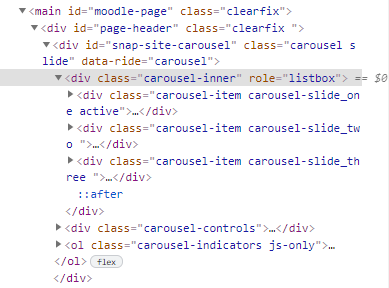
\includegraphics [scale=0.8]{Figura5.png}}
\legend{Fonte: Próprio autor}
\label{Bloco de código pertencente à página inicial do AVA, mostrando a associação das roles listbox e options}
\end{figure}

A solução para este tipo de falha de acessibilidade é encontrada no subtópico option - role \cite{world2014accessible}, que afirma a necessidade de adicionar aos elementos filhos de uma div com a role listbox o atributo role com valor option. Caso contrário, a especificação adverte que os elementos não serão corretamente mapeados pela API de acessibilidade. 

Sendo assim, o problema poderia ser resolvido refatorando o case acima como é ilustrado na figura \ref{Acréscimo das roles options para criar uma associação com a listbox}.

\begin{figure}[!h]
\centering
\caption{Acréscimo das roles options para criar uma associação com a listbox}
\fbox{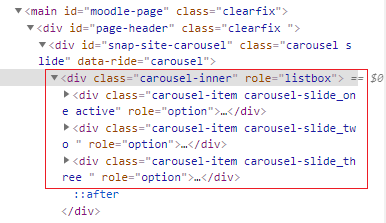
\includegraphics [scale=0.8]{Figura6.png}}
\legend{Fonte: Próprio autor}
\label{Acréscimo das roles options para criar uma associação com a listbox}
\end{figure}

\pagebreak

   \item Background and foreground colors do not have a sufficient contrast ratio.
   
Textos que não têm contraste o suficiente, além de afetarem principalmente usuários com baixa visão, também dificultam a leitura de todos os tipos de usuários. Isso pode ser notado, por exemplo, ao tentar ler algo no celular a partir de um ambiente externo e iluminado. Para resolver isso os critérios de sucesso mínimos (Nível AA) das WCAG 2.1 exigem uma taxa de contraste de pelo menos 3:1 para textos grandes – também definidos pelas diretrizes como textos maiores que 18pt se não estiverem em negrito e 14pt se estiverem. Para os demais tamanhos de texto a taxa de contraste é de 4.5:1.

Na falha de acessibilidade número 3 o teste automatizado identificou, nos elementos apontados por ele, que a taxa de contraste é menor do que as taxas exigidas pelas WCAG. Para resolver o problema, é recomendada a utilização de alguma ferramenta que mensure e redefine o contraste de um texto. Atualmente, existem várias ferramentas criadas com esse propósito, como a Chrome DevTools' Color Picker do próprio Google, a WCAG Color Contrast Checker e a Contrast Grid.

A ferramenta utilizada na pesquisa foi a Chrome DevTools’ Color Picker. Como podemos ver abaixo, na figura \ref{Apuração da taxa de contraste com o Chrome DevTools’ Color Picker}, o contraste sugerido pela WCAG no nível AA e no nível AAA seria de 4.5 e 7.0 respectivamente.

\begin{figure}[!h]
\centering
\caption{Apuração da taxa de contraste com o Chrome DevTools’ Color Picker}
\fbox{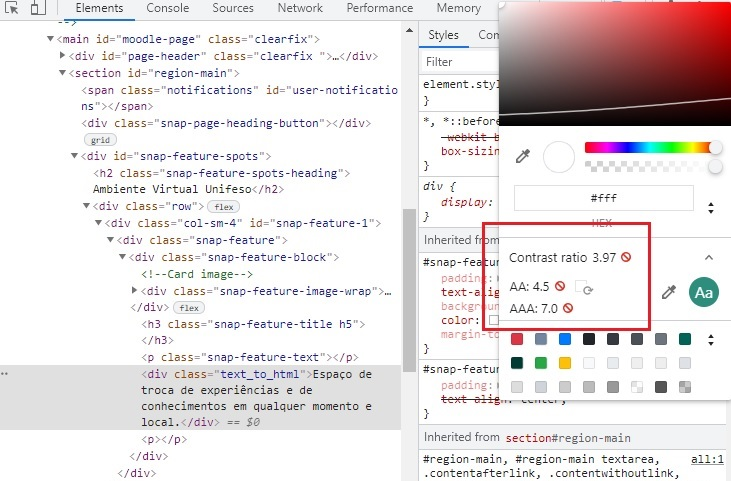
\includegraphics [scale=0.8]{Figura4.jpg}}
\legend{Fonte: Próprio autor}
\label{Apuração da taxa de contraste com o Chrome DevTools’ Color Picker}
\end{figure}

\pagebreak

 \item Id attributes on active, focusable elements are not unique
   
O atributo id no HTML, além de ser utilizado para identificar o elemento em scripts e no CSS, também responde a leitores de tela e outras tecnologias assistivas. Essas tecnologias, por esperar que o id seja único por todo o documento, acabam anunciando somente o primeiro elemento que compartilha o id em casos onde o mesmo id é definido em mais de um elemento, como informado nas Técnicas para os Critérios de Sucesso 4.1.1 \cite{cooper2010techniques}. Dessa forma, os ids duplicados tornam apenas o primeiro elemento focalizável nas navegações por tab e shift + tab, fazendo com que o usuário não consiga acessar todas as funcionalidades da página.

A falha de acessibilidade número 4 indica que há mais de um elemento compartilhando o mesmo id, como na acusação de id redundante na figura \ref{Assert do Lighthouse acusando mais de um elemento com o mesmo Id}.

\begin{figure}[!h]
\centering
\caption{Assert do Lighthouse acusando mais de um elemento com o mesmo Id}
\fbox{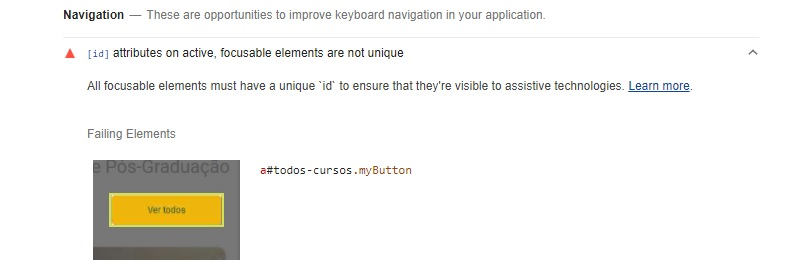
\includegraphics [scale=0.8]{Figura7.jpg}}
\legend{Fonte: Próprio autor}
\label{Assert do Lighthouse acusando mais de um elemento com o mesmo Id}
\end{figure}

\pagebreak

Para resolver esse problema é preciso identificar quais elementos têm o mesmo id (veja a figura \ref{Identificação dos elementos compartilhando o mesmo Id}) e modificá-los para que cada um tenha seu próprio id. Uma alternativa é cogitar retirar o id dos elementos e manipulá-los por suas classes.

\begin{figure}[!h]
\centering
\caption{Identificação dos elementos compartilhando o mesmo Id}
\fbox{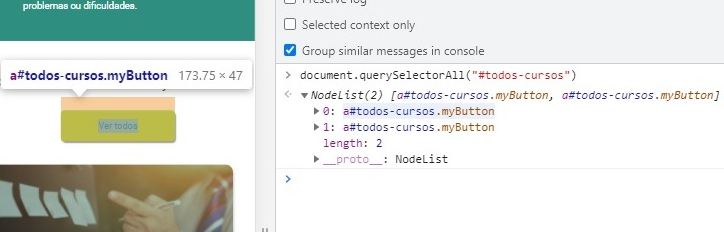
\includegraphics [scale=0.8]{Figura8.jpg}}
\legend{Fonte: Próprio autor}
\label{Identificação dos elementos compartilhando o mesmo Id}
\end{figure}

 \item Heading elements are not in a sequentially-descending order
   
Os chamados headings no HTML são definidos com as tags de <h1> até <h6> e representam os seis níveis de título de seção, assim especificado na seção 4.3.9 das recomendações do W3C para o HTML 5.2 \cite{caldwell2008web}. Um erro muito comum é utilizar esses elementos para marcar slogans, títulos alternativos e subtítulos que não pretendem representar semanticamente o título de uma nova seção, além da utilização dos seus níveis para diminuir ou aumentar o tamanho da fonte do cabeçalho. Esses enganos costumam desviar a estrutura da ordem não-sequêncial e descendente – ideal para que leitores de tela consigam navegar de heading a heading.

\begin{figure}[!h]
\centering
\caption{Análise da acessibilidade dos headings na página inicial do AVA usando a extensão Web Developer}
\fbox{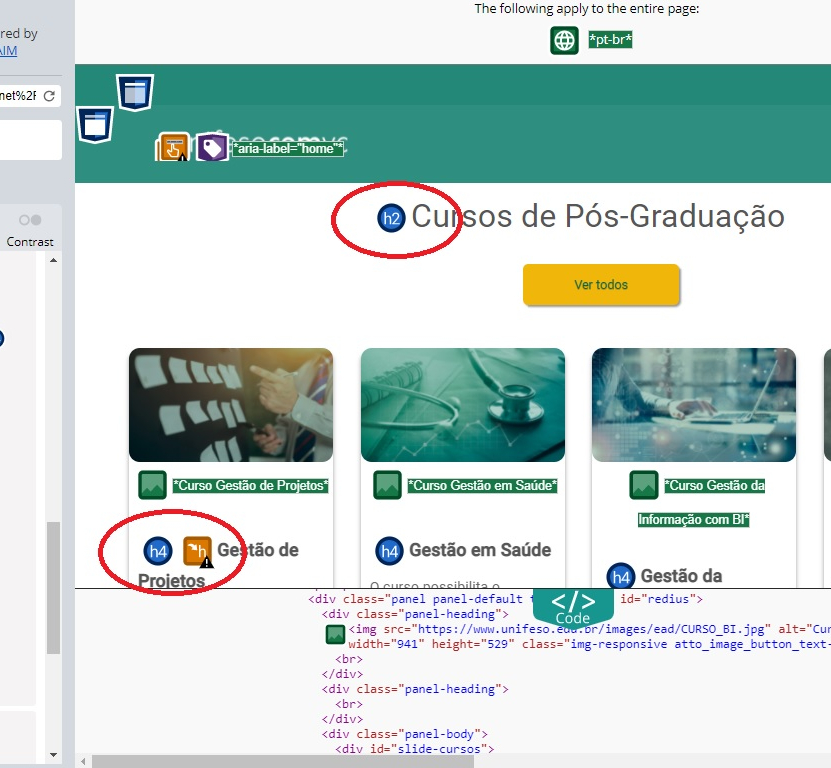
\includegraphics [scale=0.7]{Figura9.jpg}}
\legend{Fonte: Próprio autor}
\label{Análise da acessibilidade dos headings na página inicial do AVA usando a extensão Web Developer}
\end{figure}

\pagebreak

Na figura \ref{Análise da acessibilidade dos headings na página inicial do AVA usando a extensão Web Developer} acima, através da extensão Web Developer do Google Chrome, podemos visualizar que os elementos acusados pelo teste automatizado estão todos no nível h4, apesar dos headings anteriores estarem no nível h2. Para solucionar o problema, os headings devem ficar ordenados decrescente e sequencialmente, mudando os h4s da div com id “redius” para h3s e, assim, removendo o gap na sequência dos headings.

 \item Form elements do not have associated labels
   
Esta falha de acessibilidade, representada como F68 nas técnicas para o WCAG 2.0, falha dos critérios de sucesso 1.3.1 e 4.1.2 \cite{cooper2010techniques}, acontece quando não há um label associado a cada um dos elementos de controles de um formulário. Os labels garantem que esses elementos sejam anunciados apropriadamente pelos leitores de tela, além de serem utilizados por outras tecnologias assistivas para que os usuários consigam navegar através do formulário. Na figura \ref{Nenhum label associado aos inputs do form} abaixo, por exemplo, podemos notar a ausência de um label para os inputs apresentados.

\begin{figure}[!h]
\centering
\caption{Nenhum label associado aos inputs do form}
\fbox{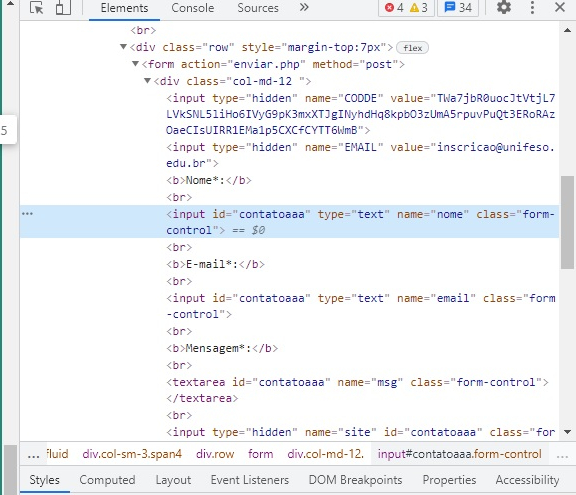
\includegraphics [scale=1.1]{Figura10.jpg}}
\legend{Fonte: Próprio autor}
\label{Nenhum label associado aos inputs do form}
\end{figure}

O método recomendado para a maioria das circunstâncias é usar o elemento label e uma associação explícita através dos atributos for e id.

 \item Image elements do not have alt attributes
   
O documento Técnicas do W3C para WCAG 2.0 contém orientações específicas sobre como atender aos critérios de sucesso das WCAG \cite{cooper2010techniques}. Ele é atualizado periodicamente, cerca de duas vezes por ano, para cobrir as práticas recomendadas mais atuais e mudanças em tecnologias e ferramentas.

A falha de acessibilidade F68 desse documento, que acusa elementos do tipo img que não têm o atributo alt, justifica que sem esse atributo um texto alternativo não pode ser computado caso a imagem tenha algum problema para ser carregada. Ainda que algumas tecnologias assistivas tentem compensar a falta do texto alternativo lendo o nome do arquivo da imagem, ainda é insuficiente na medida em que nomes de arquivos geralmente não são descritivos.

Nos casos em que a imagem atua apenas como decoração e não fornece nenhum conteúdo útil de fato, ainda é uma boa prática atribuir o atributo alt = "" (vazio) para remover a falha da árvore de acessibilidade.

Embora existam os atributos WAI-ARIA que podem ser usados para fornecer um texto alternativo, desde que sejam compatíveis com a acessibilidade, ainda é recomendado pelas Técnicas do W3C para WCAG 2.0 o atributo alt como a forma preferida de resolver essa falha de acessibidade.

\begin{figure}[!h]
\centering
\caption{Ausência do atributo alt na tag img}
\fbox{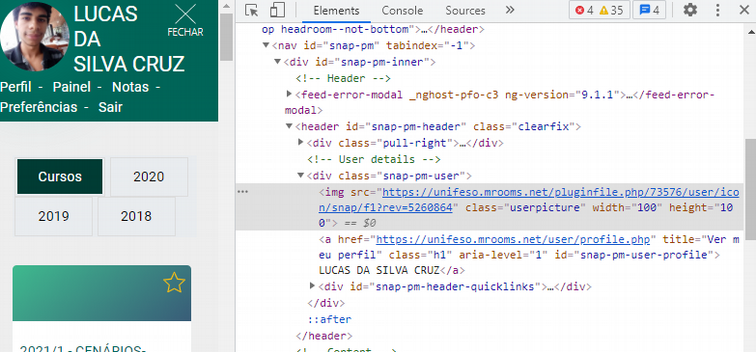
\includegraphics [scale=0.8]{Figura11.png}}
\legend{Fonte: Próprio autor}
\label{Ausência do atributo alt na tag img}
\end{figure}

Na figura \ref{Ausência do atributo alt na tag img} acima podemos perceber a ausência do atributo alt, aria-label ou aria-labelledby associado a algum id. Como também é um elemento conteudístico – que representa a imagem de perfil de algum usuário – é recomendado, para solucionar o problema, uma simples adição do atributo alt com um valor descritivo da imagem.


 \item Object elements do not have alt text
   
O elemento object representa um recurso externo que pode ser tratado como uma imagem, um contexto de navegação aninhado ou um recurso a ser provido por um plugin. \cite{htmldoc}. Dessa forma, a mídia desse elemento só está disponível para o usuário quando ela não é renderizada pelo agente do usuário – o agente pode não oferecer suporte à tecnologia de mídia ou o usuário o instruiu a não renderizar essa tecnologia, segundo a Falha de acessibilidade H53 \cite{cooper2010techniques}.

Nos casos em que os leitores de tela e outras tecnologias assistivas não conseguem interpretar o conteúdo do elemento object, ele deve oferecer um texto alternativo que permita transmitir o significado do elemento para os usuários. Essa falha H53 recomenda que o texto alternativo seja inserido no próprio corpo do elemento, como exemplificado abaixo:

\begin{center}
\begin{minipage}{10cm}
\begin{verbatim}
<object type="application/pdf" data="/report.pdf">
    2019 Web Accessibility Report
</object>
\end{verbatim}
\end{minipage}
\end{center}

\begin{figure}[!h]
\centering
\caption{Ausência do atributo alt no corpo do elemento object}
\fbox{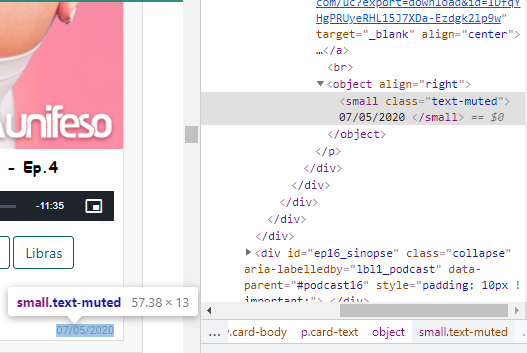
\includegraphics [scale=0.9]{Figura12.png}}
\legend{Fonte: Próprio autor}
\label{Ausência do atributo alt no corpo do elemento object}
\end{figure}

Na figura \ref{Ausência do atributo alt no corpo do elemento object} acima pode ser notado que não há um texto alternativo inserido diretamente no corpo do elemento object, por isso ele é acusado com uma falha de acessibilidade. A solução recomendada para este tipo de problema é simplesmente adicionar um texto descritivo seu corpo.

 \item Frame or iframe elements do not have a title
   
A técnica H64 demonstra o uso do atributo title nos elementos frame e iframe: “O atributo title fornece um label para o frame e assim os usuários podem determinar qual frame querem entrar e explorar em detalhes.” \cite{cooper2010techniques}.

Os leitores de tela e outras tecnologias precisam desse atributo nos frames ou iframes para descrever o conteúdo deles. Sem o atributo, navegar por esses elementos pode se tornar muito rapidamente difícil e confuso para o usuário de alguma tecnologia assistiva.

\begin{figure}[!h]
\centering
\caption{Ferramenta Lighthouse acusando elemento iframe de não ter atributo title}
\fbox{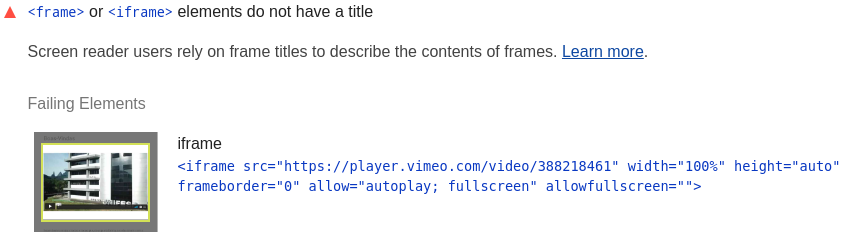
\includegraphics [scale=0.5]{Figura13.png}}
\legend{Fonte: Próprio autor}
\label{Ferramenta Lighthouse acusando elemento iframe de não ter atributo title}
\end{figure}

\pagebreak

 \item ARIA progressbar elements do not have accessible names
   
“A role progressbar indica que a requisição do usuário foi realizada e o aplicativo está progredindo para concluir a ação solicitada.” \cite{world2014accessible}. Quando esse elemento não tem um nome acessível, os leitores de tela e outras tecnologias assitivas o anunciam com um nome genérico, inutilizável para o usuário que depende das tecnologias. Como por exemplo no elemento abaixo, ilustrado na figura \ref{Lighthouse acusando elemento com nome inacessível para leitores de tela}, acusado pelo Lighthouse com essa falha:

\begin{figure}[!h]
\centering
\caption{Lighthouse acusando elemento com nome inacessível para leitores de tela}
\fbox{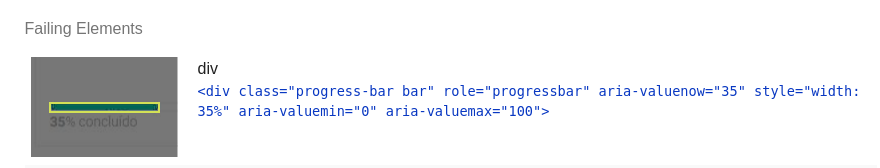
\includegraphics [scale=0.5]{Figura14.png}}
\legend{Fonte: Próprio autor}
\label{Lighthouse acusando elemento com nome inacessível para leitores de tela}
\end{figure}

Uma das formas de resolver esse problema, quando não queremos que o nome do elemento seja visível na página, é através do atributo aria-label, que tem justamente o propósito de informar um nome mais apropriado. O código acima poderia, então, ser refatorado da seguinte maneira:

\begin{center}
\begin{minipage}{10cm}
\begin{verbatim}
<div class="progress-bar bar" role="progressbar" 
aria-label="nome-anunciado-pelas-tecs-assistivas" 
aria-valuenow="35" style="width: 35%" 
aria-valuemin="0" aria-valuemax="100">
\end{verbatim}
\end{minipage}
\end{center}

 \item Links do not have a discernible name
   
Um link deve sempre prover no seu conteúdo um texto descritivo. “A descrição permite o usuário destinguir esse link de outros na página e também determinar se ele deve ou não seguir o link uma vez que a URI de destino geralmente não é suficientemente descritiva” \cite{cooper2010techniques}.

O documento também antecipa as situações onde uma imagem é o único conteúdo de um link. Nesse caso, ele diz que a alternativa em texto para imagem – atributo alt – descreve a função exclusiva do link.

A figura \ref{Um elemento de link que não fornece texto descritivo} exibe o trecho de código onde o Lighthouse identificou o problema. Como podemos ver, não há um texto descritivo contido diretamente no link de id “snap-pm-trigger”. Apesar de ter uma imagem, também não é fornecido um  atributo alt que serviria como descrição da função do link.

\begin{figure}[!h]
\centering
\caption{Um elemento de link que não fornece texto descritivo}
\fbox{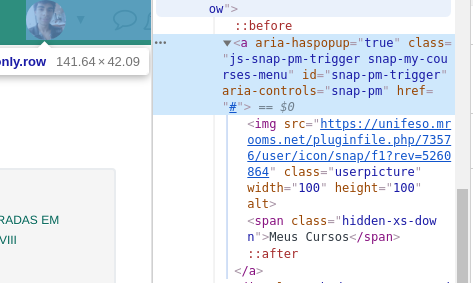
\includegraphics [scale=0.8]{Figura15.png}}
\legend{Fonte: Próprio autor}
\label{Um elemento de link que não fornece texto descritivo}
\end{figure}

Para resolver esse problema basta adicionar algum valor ao atributo alt da tag img. Alternativamente, também é possível utilizar a aria-label, considerando que é uma situação muito próxima da analisada anteriormente no ponto 5.2.10, onde era necessário um texto descritivo para o elemento sem que ele fosse renderizado de fato na página. A figura \ref{Acréscimo de aria-label a um link sem texto descritivo} representa a implementação dessa solução.

\begin{figure}[!h]
\centering
\caption{Acréscimo de aria-label a um link sem texto descritivo}
\fbox{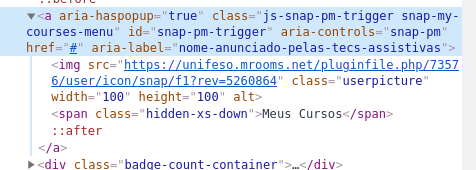
\includegraphics [scale=0.8]{Figura16.png}}
\legend{Fonte: Próprio autor}
\label{Acréscimo de aria-label a um link sem texto descritivo}
\end{figure}

\pagebreak

 \item Lists do not contain only <li> elements and script supporting elements (<script> and <template>)
   
Uma prática bastante comum na manipulação do HTML que infelizmente gera uma série de problemas de acessibilidade é a não utilização da semântica da linguagem (também conhecida como POSH, ou \textit{Plain Old Semantic HTML}). Embora seja possível nas combinações de CSS com o JavaScript fazer com que qualquer elemento HTML se comporte da forma que quisermos, é muito provável que as propriedades built-in dos elementos – já embutidos com padrões de acessibilidade pelo teclado – não sejam consideradas na versão não-semântica do HTML. Um bom exemplo dessa prática é quando usam o elemento div para representar um botão sobrescrevendo os estilos padrão dele. Embora visualmente fique semelhante a um botão, as propriedades padrão não serão as mesmas. Isso faz com que as tecnologias assistivas anunciem os elementos de forma errada para os usuários com alguma deficiência, além de encontrar problemas para navegar entre os elementos.

Uma lista pode ser de definição, ordenada ou desordenada. Quando a lista é ordenada (elemento ol) ou desordenada (elemento ul) todos os seus filhos devem ser um list item  (elemento li). É por isso que, como  afirmado na técnica H48, “quando uma marcação é usada para formatar itens visualmente como uma lista, mas  não representam o relacionamento da lista, os usuários (de alguma tecnologia assistiva) têm dificuldade para navegar pelas informações” \cite{cooper2010techniques}.

Nas figuras \ref{Estrutura do AVA acusado pelo Lighthouse com problema de acessibilidade: um  elemento ul mantendo uma div como filha além dos elementos lis apropriados} e \ref{Div representando um item visual de carregamento} abaixo podemos perceber, analisando os trechos de código denunciados pela ferramenta Lighthouse, que a div contida dentro da ul forma, na verdade, uma animação de carregamento para o usuário a espera de alguma requisição. Como não é semanticamente adequada a uma lista, a solução recomendada é de mover a div acima ou abaixo dela e usar CSS para reposicionar o elemento, de forma que não altere o visual atual da página mas entre em conformidade com o POSH.

\begin{figure}[!h]
\centering
\caption{Estrutura do AVA acusado pelo Lighthouse com problema de acessibilidade: um  elemento ul mantendo uma div como filha além dos elementos lis apropriados}
\fbox{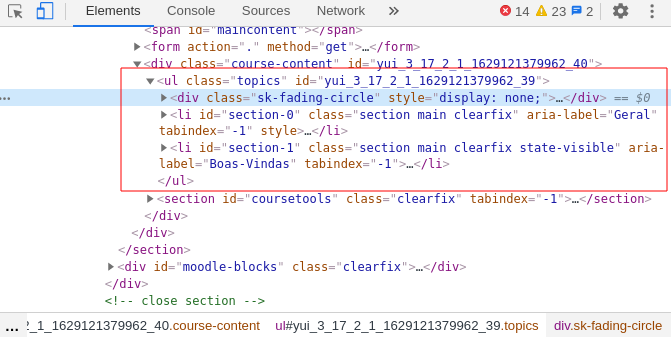
\includegraphics [scale=0.8]{Figura17.png}}
\legend{Fonte: Próprio autor}
\label{Estrutura do AVA acusado pelo Lighthouse com problema de acessibilidade: um  elemento ul mantendo uma div como filha além dos elementos lis apropriados}
\end{figure}

\begin{figure}[!h]
\centering
\caption{Div representando um item visual de carregamento}
\fbox{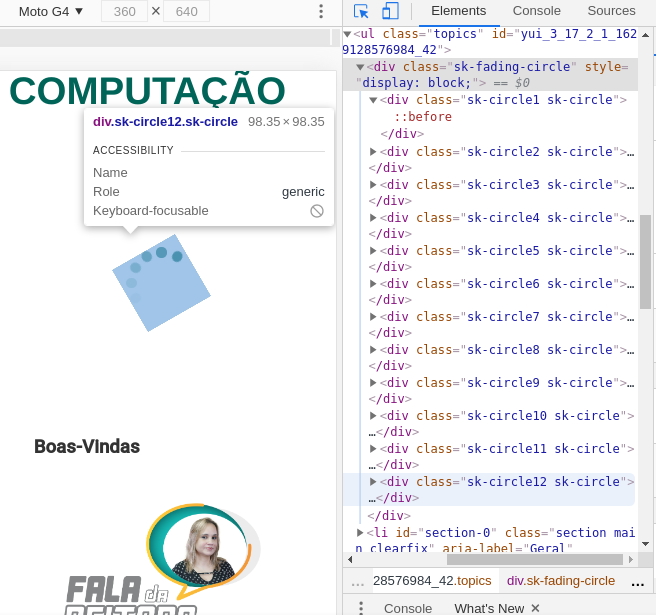
\includegraphics [scale=0.7]{Figura18.png}}
\legend{Fonte: Próprio autor}
\label{Div representando um item visual de carregamento}
\end{figure}


\end{itemize}

% ----------------------------------------------------------
% Considerações Finais
% ----------------------------------------------------------
\chapter{CONCLUSÕES}

Na métrica de desempenho e boa experiência de usuário com a acessibilidade de um site ou sistema da web, provida pelo Google Lighthouse, a classificação do AVA da Unifeso está em laranja – pontuação de 50 a 89 – que define o nível de acessibilidade do ambiente como “precisa de melhoria”. O Lighthouse também recomenda a coloração verde, que classifica o sistema com “bom nível de acessibilidade”, para uma experiência de usuário satisfatória e esperada da Web – projetada para ser utilizada por qualquer pessoa e que fornece diretrizes de acessibilidade que tornam o conteúdo na internet acessível a um maior número de pessoas com deficiência quando implementadas.

Este trabalho foi um estudo de caso com o intuito de tornar o AVA da Unifeso mais acessível, identificando suas vulnerabilidades e propondo melhorias nos pontos chaves que mais afetam as páginas do sistema. Foi realizado um levantamento das principais tecnologias e stacks envolvidas na realização de testes automatizados de acessibilidade, além dos métodos e das principais abordagens utilizadas para testar a acessibilidade manualmente – complementando a análise com aspectos que somente os testes automatizados não conseguem identificar. A principal ferramenta escolhida para fazer os testes automatizados foi o próprio Lighthouse, que recentemente incorporou o axe-core como uma de suas bibliotecas e atualmente está integrado ao Chrome DevTools e disponível no Google Chrome a partir da versão 60.

Além das estatísticas que a pesquisa levantou, que ajudam a identificar os problemas chaves de acessibilidade, mais frequentes e como estão distribuídos, também foram encontradas 12 propostas de soluções que impactariam consideravelmente na pontuação de acessibilidade do AVA, inserindo a plataforma na classificação verde – considerada ideal pelo Google Lighthouse.

\chapter{TRABALHOS FUTUROS}

\begin{itemize}

    \item Checagem de SEO com Lighthouse e impactos da acessibilidade no rankeamento do Google: Estatísticas do antes e depois da melhoria de acessibilidade do AVA da Feso
    
Com as estatísticas de acessibilidade do AVA levantadas e documentadas antes das propostas de melhorias sugeridas nesse trabalho terem sido implementadas, sabendo-se que o Google Lighthouse também faz auditoria de SEO, uma nova análise automatizada após a realização dessas melhorias demonstraria a relação do nível de acessibilidade com o rankeamento das páginas pelo Google

\end{itemize}

% ----------------------------------------------------------
% ELEMENTOS PÓS-TEXTUAIS
% ----------------------------------------------------------
\postextual
% ----------------------------------------------------------

% ----------------------------------------------------------
% Referências bibliográficas
% ----------------------------------------------------------
\bibliography{bibliografia}
% ---


% ----------------------------------------------------------
% Apêndices
% ----------------------------------------------------------

% ---
% Inicia os apêndices
% ---
%\begin{apendicesenv}
	
	% Imprime uma página indicando o início dos apêndices
	%\partapendices
	
% ----------------------------------------------------------
%\chapter{Exemplo}
% ----------------------------------------------------------
	
%\end{apendicesenv}
% ---

% ----------------------------------------------------------
% Anexos
% ----------------------------------------------------------

% ---
% Inicia os anexos
% ---
%\begin{anexosenv}
	
	% Imprime uma página indicando o início dos anexos
	%\partanexos
	
	% ---
    %\chapter{Exemplo}
    % ---
	
%\end{anexosenv}

\end{document}
